\chapter{Results}

%Template:
%Result name
%Why it is generated
%Result figures

Results produced in this thesis stem from the final two experiments.
First, from the iterative re-training of the neural network, then from using the iterative re-training to create a classification tree.
As the experiments did varying amounts of repeating steps that can magnify potential errors in the final results, the results are presented in a broad view. 

%Results to be generated:
%Iterative
\section{Iterative re-training results}
\label{res:iter}
This section goes through the entire result dataset for \cref{ex:iter-retrain}, in various forms.
The parameters used in the various examples are:

\begin{itemize}
    \item Function option, -2, -1, 0, 1, 2, 3
    \item Iteration threshold: 0.5, 0.6, 0.7, 0.8, 0.9
\end{itemize}{}
An explanation of these values is listed in \cref{ex:iter-retrain:params}.
The results are based on parsing the entire dataset with the neural network created on each iteration of the re-training process.
As the results can be broken up into three general types, the resulting graphs are broken up into different groups where appropriate.

%Size of largest cluster for each combination, as number of iterations increases, compare each threshold as their iterations were similar
\subsection{Size of clusters over the iterations}

\begin{figure}  % order of priority: h here, t top, b bottom, p page
  \centering
  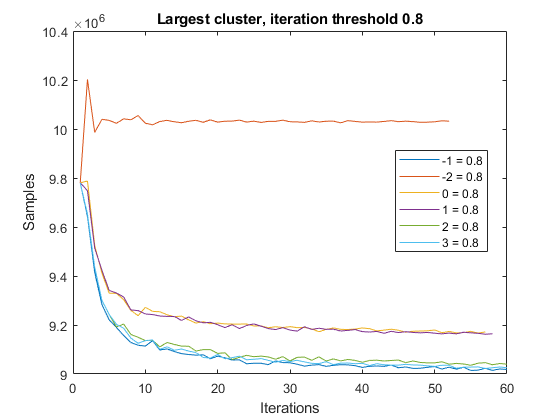
\includegraphics[width=.7\textwidth]{figures/largest-0.8.png}
  \caption{Largest cluster over the iterations, with 0.8 iteration threshold}
  \label{fig:iter:largestcluster0.8}
\end{figure}

\begin{figure}
    \centering
    \begin{subfigure}[b]{.45\textwidth}
        \centering
        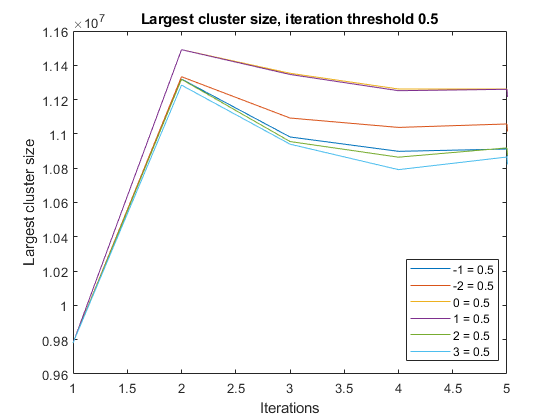
\includegraphics[width=\textwidth]{figures/largest-0.5.png}
        \caption{0.5 iteration threshold}
        \label{sfig:iter:largestcluster0.5}
    \end{subfigure}
    \hfill
    \begin{subfigure}[b]{.45\textwidth}
        \centering
        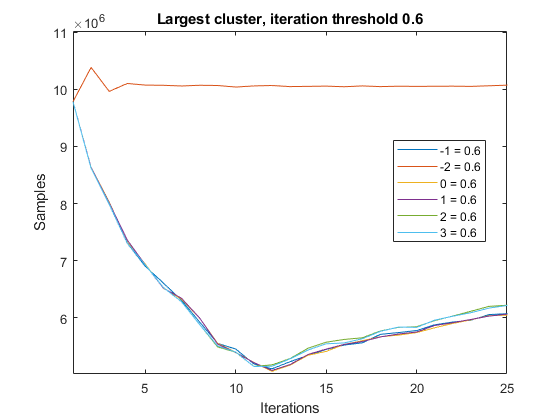
\includegraphics[width=\textwidth]{figures/largest-0.6.png}
        \caption{0.6 iteration threshold}
        \label{sfig:iter:largestcluster0.6}
    \end{subfigure}
    \caption{Largest cluster over the iterations, with 0.5 and 0.6 iteration threshold}
    \label{fig:iter:largestcluster0.50.6}
\end{figure}

\begin{figure}
    \centering
    \begin{subfigure}[b]{.45\textwidth}
        \centering
        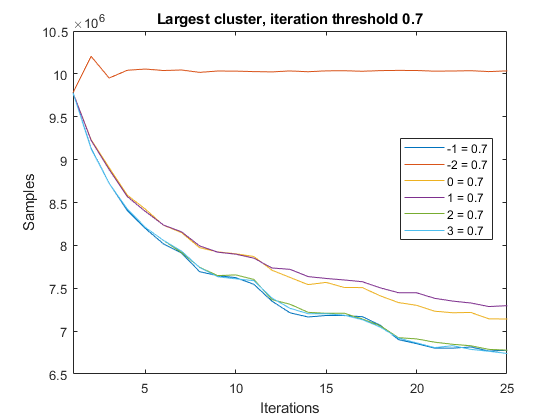
\includegraphics[width=\textwidth]{figures/largest-0.7.png}
        \caption{0.7 iteration threshold}
        \label{sfig:iter:largestcluster0.7}
    \end{subfigure}
    \hfill
    \begin{subfigure}[b]{.45\textwidth}
        \centering
        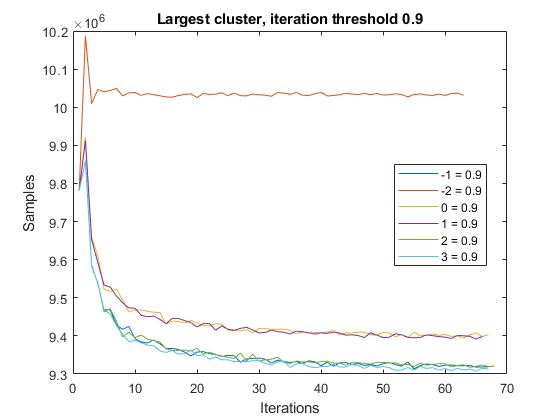
\includegraphics[width=\textwidth]{figures/largest-0.9.png}
        \caption{0.9 iteration threshold}
        \label{sfig:iter:largestcluster0.9}
    \end{subfigure}
    \caption{Largest cluster over the iterations, with 0.7 and 0.9 iteration threshold}
    \label{fig:iter:largestcluster0.70.9}
\end{figure}

\cref{fig:iter:largestcluster0.8}, \cref{fig:iter:largestcluster0.50.6}, and \cref{fig:iter:largestcluster0.70.9} detail the size of the result clusters as the number of iterations increases.

As the size of the clusters is the most straightforward value to track across the iterations, it is listed first.
Partial cluster size results were used to make the decision on which iteration threshold to pick for \cref{ex:tree}.

%Values of the highest classification, how certain the network becomes over the iterations in its results
\subsection{Value of the highest classifications over the iterations}
The value of the highest classification is also a vital characteristic to track across the iterations.
Should the cluster size vary wildly with the highest classification value remaining the same, it could indicate a heavy overfit in the network and flimsy reasoning for the cluster separation.
Besides, the goal of the iterative re-training is to reduce the uncertainty of the classification, which can be tracked by following the highest classification values for the given samples.

Following the iteration threshold parameter, the most critical change in the highest classification happens when the iteration threshold is reached.
\cref{fig:iter:iterbelow0.8}, \cref{fig:iter:iterbelow0.50.6}, and \cref{fig:iter:iterbelow0.70.9} present the number of samples that are below the iteration threshold over the course of the iterative re-training.

\begin{figure}  % order of priority: h here, t top, b bottom, p page
  \centering
  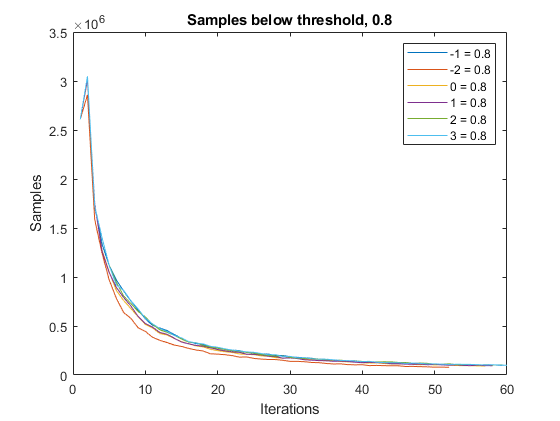
\includegraphics[width=.7\textwidth]{figures/iterbelow-0.8.png}
  \caption{Samples below iteration threshold, with parameter set to 0.8.}
  \label{fig:iter:iterbelow0.8}
\end{figure}

\begin{figure}
    \centering
    \begin{subfigure}[b]{.45\textwidth}
        \centering
        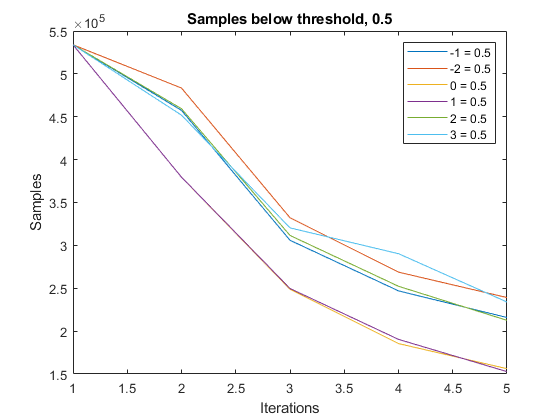
\includegraphics[width=\textwidth]{figures/iterbelow-0.5.png}
        \caption{0.5 iteration threshold}
        \label{sfig:iter:iterbelow0.5}
    \end{subfigure}
    \hfill
    \begin{subfigure}[b]{.45\textwidth}
        \centering
        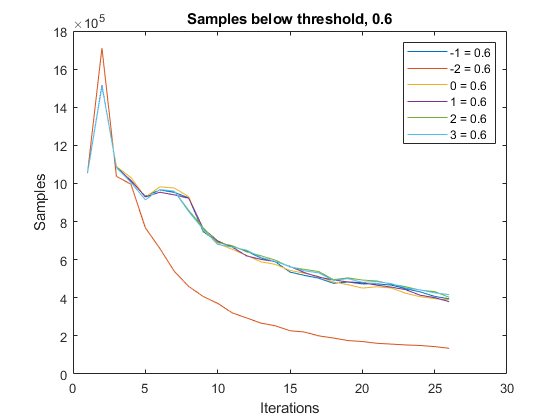
\includegraphics[width=\textwidth]{figures/iterbelow-0.6.png}
        \caption{0.6 iteration threshold}
        \label{sfig:iter:iterbelow0.6}
    \end{subfigure}
    \caption{Samples below iteration threshold, with parameter set to 0.5 and 0.6}
    \label{fig:iter:iterbelow0.50.6}
\end{figure}

\begin{figure}
    \centering
    \begin{subfigure}[b]{.45\textwidth}
        \centering
        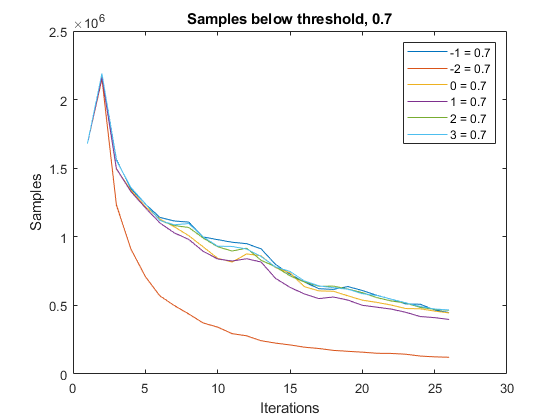
\includegraphics[width=\textwidth]{figures/iterbelow-0.7.png}
        \caption{0.7 iteration threshold}
        \label{sfig:iter:iterbelow0.7}
    \end{subfigure}
    \hfill
    \begin{subfigure}[b]{.45\textwidth}
        \centering
        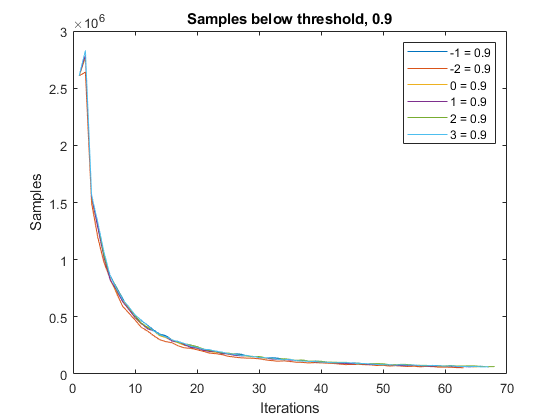
\includegraphics[width=\textwidth]{figures/iterbelow-0.9.png}
        \caption{0.9 iteration threshold}
        \label{sfig:iter:iterbelow0.9}
    \end{subfigure}
    \caption{Samples below iteration threshold, with parameter set to 0.7 and 0.9.}
    \label{fig:iter:iterbelow0.70.9}
\end{figure}

%Variation from first network result over the iterations
\subsection{Variation between first iteration and the following iterations}

The goal of the re-training process is to train the network more, faster than just using the entire dataset and a big data center worth of hardware.
However, significant variations throughout the entire training process can indicate that the parameters do not converge into a particular cluster group.
While the first iteration is expected not to be the perfect network immediately, it is still expected to be a general approximation of the problem, and significant changes to the initial cluster group can indicate problems in the combinations.

Only changes of 0.1 or more are tracked to represent the change as something more significant than a minor rounding error. 
\cref{fig:iter:varfirst0.8}, \cref{fig:iter:varfirst0.50.6}, and \cref{fig:iter:largestcluster0.70.9} present the number of samples that had a change in the highest class.


\begin{figure}  % order of priority: h here, t top, b bottom, p page
  \centering
  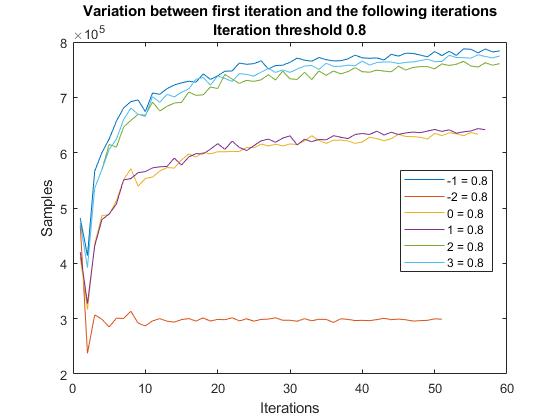
\includegraphics[width=.7\textwidth]{figures/varfirst-0.8.png}
  \caption{Variation between first and next iterations, with 0.8 iteration threshold}
  \label{fig:iter:varfirst0.8}
\end{figure}

\begin{figure}
    \centering
    \begin{subfigure}[b]{.45\textwidth}
        \centering
        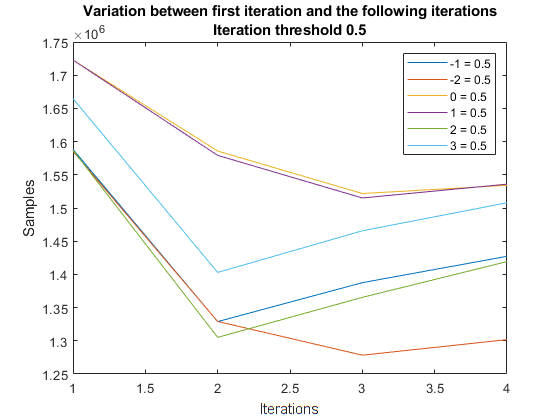
\includegraphics[width=\textwidth]{figures/varfirst-0.5.png}
        \caption{0.5 iteration threshold}
        \label{sfig:iter:varfirst0.5}
    \end{subfigure}
    \hfill
    \begin{subfigure}[b]{.45\textwidth}
        \centering
        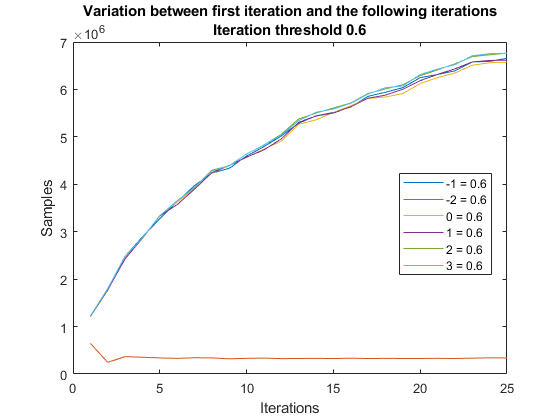
\includegraphics[width=\textwidth]{figures/varfirst-0.6.png}
        \caption{0.6 iteration threshold}
        \label{sfig:iter:varfirst0.6}
    \end{subfigure}
    \caption{Variation between first and next iterations, with 0.5 and 0.6 iteration threshold}
    \label{fig:iter:varfirst0.50.6}
\end{figure}

\begin{figure}
    \centering
    \begin{subfigure}[b]{.45\textwidth}
        \centering
        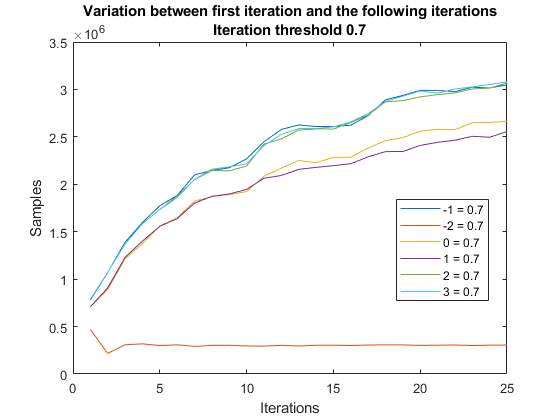
\includegraphics[width=\textwidth]{figures/varfirst-0.7.png}
        \caption{0.7 iteration threshold}
        \label{sfig:iter:varfirst0.7}
    \end{subfigure}
    \hfill
    \begin{subfigure}[b]{.45\textwidth}
        \centering
        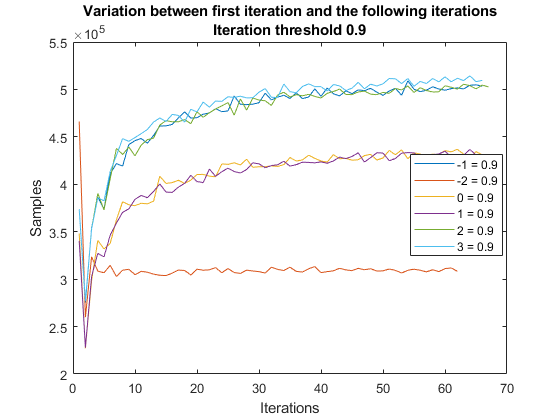
\includegraphics[width=\textwidth]{figures/varfirst-0.9.png}
        \caption{0.9 iteration threshold}
        \label{sfig:iter:varfirst0.9}
    \end{subfigure}
    \caption{Variation between first and next iterations, with 0.7 and 0.9 iteration threshold}
    \label{fig:iter:varfirst0.70.9}
\end{figure}

%Variations between the networks, array comparison?, pick one or two of the combinations for this 0/1, 2/3, then -1 and -2
%Array is too big/too many combinations, compare previous/next
\subsection{Variation between neighbor iterations}
In a similar manner to the previous section, this section aims to compare the neighboring iterations with each other.
While significant variations could remain present when comparing the first iteration with the others after new information was gained, comparing neighbors serves to localize the comparison.
If the variation between the iterations remains significant, it could indicate that the networks never converge into a particular classification, and just keep juggling samples between the classes.

The result in this section mimics the previous section, only with a different set of results.
Only changes of 0.1 or more are tracked to represent the change as something more significant than a minor rounding error. 
\cref{fig:iter:varneigh0.8}, \cref{fig:iter:varneigh0.50.6}, and \cref{fig:iter:varneigh0.70.9} present the number of samples that had a change in the highest class.

\begin{figure}  % order of priority: h here, t top, b bottom, p page
  \centering
  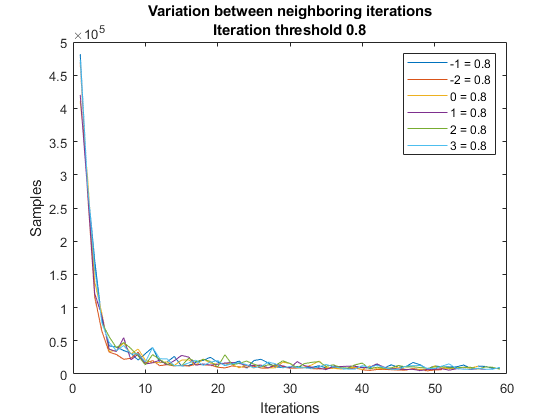
\includegraphics[width=.7\textwidth]{figures/varneigh-0.8.png}
  \caption{Variation between neighbor iterations, with 0.8 iteration threshold}
  \label{fig:iter:varneigh0.8}
\end{figure}

\begin{figure}
    \centering
    \begin{subfigure}[b]{.45\textwidth}
        \centering
        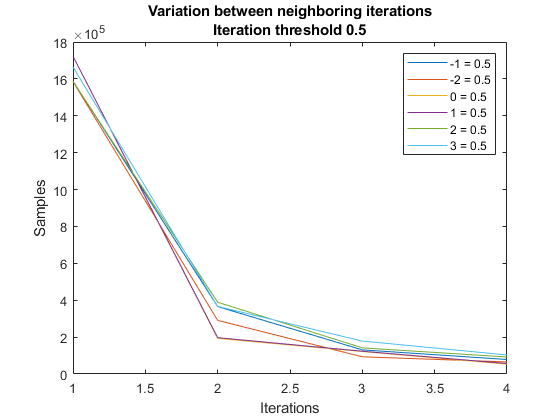
\includegraphics[width=\textwidth]{figures/varneigh-0.5.png}
        \caption{0.5 iteration threshold}
        \label{sfig:iter:varneigh0.5}
    \end{subfigure}
    \hfill
    \begin{subfigure}[b]{.45\textwidth}
        \centering
        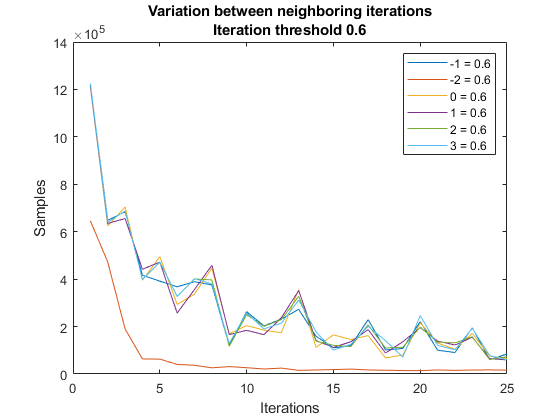
\includegraphics[width=\textwidth]{figures/varneigh-0.6.png}
        \caption{0.6 iteration threshold}
        \label{sfig:iter:varneigh0.6}
    \end{subfigure}
    \caption{Variation between neighbor iterations, with 0.5 and 0.6 iteration threshold}
    \label{fig:iter:varneigh0.50.6}
\end{figure}

\begin{figure}
    \centering
    \begin{subfigure}[b]{.45\textwidth}
        \centering
        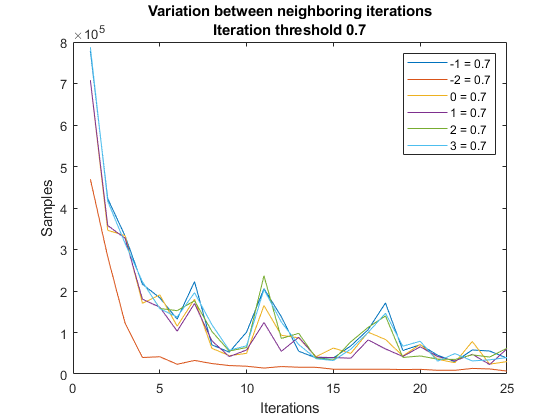
\includegraphics[width=\textwidth]{figures/varneigh-0.7.png}
        \caption{0.7 iteration threshold}
        \label{sfig:iter:varneigh0.7}
    \end{subfigure}
    \hfill
    \begin{subfigure}[b]{.45\textwidth}
        \centering
        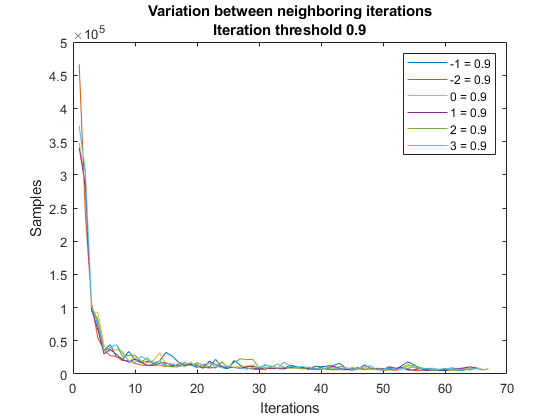
\includegraphics[width=\textwidth]{figures/varneigh-0.9.png}
        \caption{0.9 iteration threshold}
        \label{sfig:iter:varneigh0.9}
    \end{subfigure}
    \caption{Variation between neighbor iterations, with 0.7 and 0.9 iteration threshold}
    \label{fig:iter:varneigh0.70.9}
\end{figure}

%Iteration spacing between training, 22, 44, 80 etc sort of deal, convert hitlist into increasing number
\subsection{Number of sample files between training iterations}
Finally, an important variable to analyze is the effect of the iterative re-training over time, as the dataset is processed.
While in the beginning little is known about the dataset, as more and more information is gleaned on the dataset, it is expected that the network becomes more and more capable of handling information it has not seen yet.
Should the number of files between iterations not change, or even go down, it could indicate that the network loses information in the training process, or that the samples have a meager amount of common features between each other.
\cref{fig:iter:iterfiles0.8}, \cref{fig:iter:iterfiles0.50.6}, and \cref{fig:iter:iterfiles0.70.9} show the change in number of files used by the various function options over the course of the iterative re-training process.

\begin{figure}  % order of priority: h here, t top, b bottom, p page
  \centering
  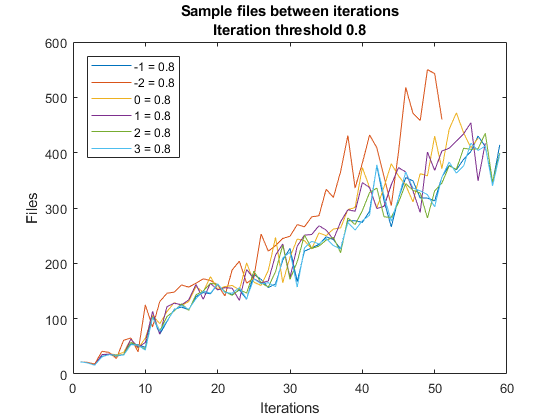
\includegraphics[width=.7\textwidth]{figures/iterfiles-0.8.png}
  \caption{Change in number of sample files between iterations, with 0.8 iteration threshold}
  \label{fig:iter:iterfiles0.8}
\end{figure}

\begin{figure}
    \centering
    \begin{subfigure}[b]{.45\textwidth}
        \centering
        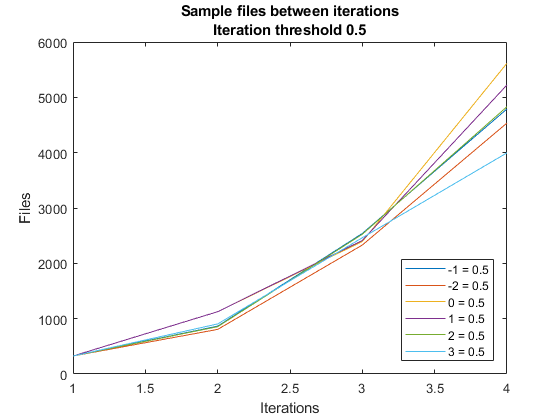
\includegraphics[width=\textwidth]{figures/iterfiles-0.5.png}
        \caption{0.5 iteration threshold}
        \label{sfig:iter:iterfiles0.5}
    \end{subfigure}
    \hfill
    \begin{subfigure}[b]{.45\textwidth}
        \centering
        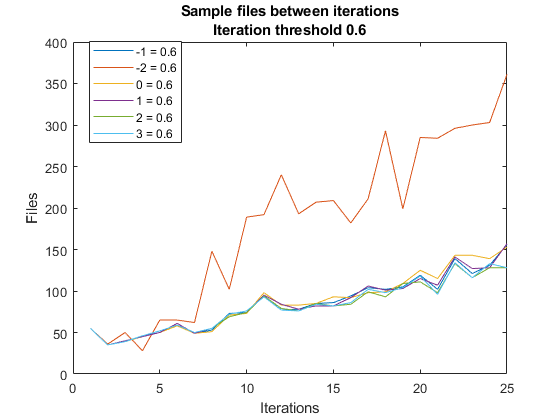
\includegraphics[width=\textwidth]{figures/iterfiles-0.6.png}
        \caption{0.6 iteration threshold}
        \label{sfig:iter:iterfiles0.6}
    \end{subfigure}
    \caption{Change in number of sample files between iterations, with 0.5 and 0.6 iteration threshold}
    \label{fig:iter:iterfiles0.50.6}
\end{figure}

\begin{figure}
    \centering
    \begin{subfigure}[b]{.45\textwidth}
        \centering
        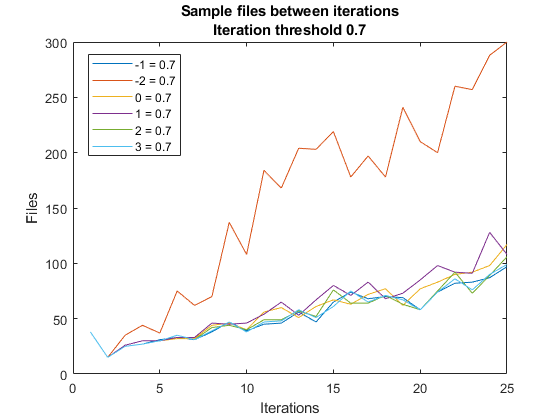
\includegraphics[width=\textwidth]{figures/iterfiles-0.7.png}
        \caption{0.7 iteration threshold}
        \label{sfig:iter:iterfiles0.7}
    \end{subfigure}
    \hfill
    \begin{subfigure}[b]{.45\textwidth}
        \centering
        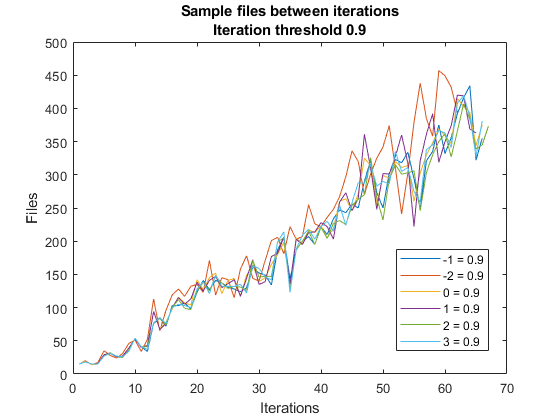
\includegraphics[width=\textwidth]{figures/iterfiles-0.9.png}
        \caption{0.9 iteration threshold}
        \label{sfig:iter:iterfiles0.9}
    \end{subfigure}
    \caption{Change in number of sample files between iterations, with 0.7 and 0.9 iteration threshold}
    \label{fig:iter:iterfiles0.70.9}
\end{figure}

%Tree
\section{Tree results}
\label{res:tree}
This section goes through the entire result dataset for \cref{ex:tree}.
The parameters used in the various examples are:

\begin{itemize}
    \item Function option, -3, -2, -1, 0, 1, 2, 3
    \item Cache threshold: 0.5, (0.2, 0.3, and 0.4 with -3 only)
\end{itemize}{}

An explanation of these values is listed in \cref{ex:treeparam}.
As the results are far more numerous in this section, processing of these results using all of the neural networks would take an excessive amount of time.
Therefore, a compromise was used in the form of utilizing the classification results generated for the caching process.

In addition to the standard comparison of function options, \cref{ex:tree} included a control group that did not use iterative re-training.
Results of that particular group of tests are included in the last subsection.

%Size of largest cache in tree, descending, max of 20? (just measure file size of next in line)
\subsection{Cache size of the nodes in the tree}
Among the most relevant results for the tree generation process are the sizes of the caches used to train the various nodes in the tree.
Some function options could distribute their dataset more evenly, while others could heavily lean towards putting all samples in just one class.
Furthermore, the control groups could provide the same or better results than the developed experiment, casting doubt into the need for the extra processing steps.

\begin{figure}
    \centering
    \begin{subfigure}[b]{.45\textwidth}
        \centering
        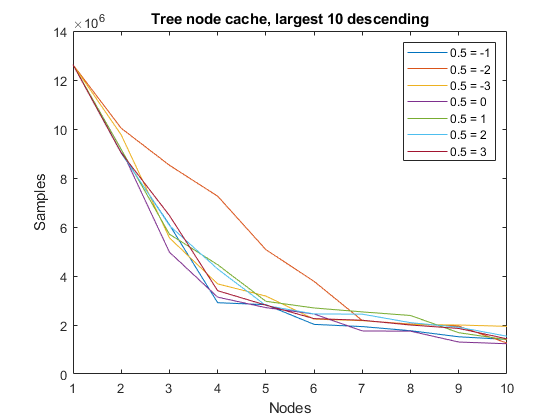
\includegraphics[width=\textwidth]{figures/treenodecache-10.png}
        \caption{Largest 10 caches}
        \label{sfig:tree:treecache10}
    \end{subfigure}
    \hfill
    \begin{subfigure}[b]{.45\textwidth}
        \centering
        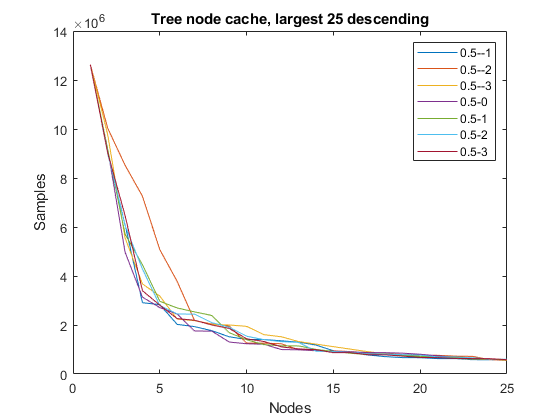
\includegraphics[width=\textwidth]{figures/treenodecache-25.png}
        \caption{Largest 25 caches}
        \label{sfig:tree:treecache25}
    \end{subfigure}
    \caption{Largest tree node caches in descending order. All start from full dataset.}
    \label{fig:tree:treecache}
\end{figure}

\cref{fig:tree:treecache} shows the size of the cache, descending from the largest to smallest.
As each tree can have different trees putting samples in differently named clusters, the names of the clusters are ignored.

%Number of iterations for each cluster in tree, excluding root node, descending, exists in metadata
%Also include iteration count in some form here
\subsection{Re-training iterations throughout the trees}
Using the iterative re-training process in the tree generation is a very dynamic way to test the method on a vast number of sample combinations.
However, it can also show signs of failure if it takes more and more iterations to train each next node in the tree.
Iterative re-training adds a constant number of samples per iteration to the training process, which can, in the worst case, end up using the entire dataset.

\begin{figure}
    \centering
    \begin{subfigure}[b]{.45\textwidth}
        \centering
        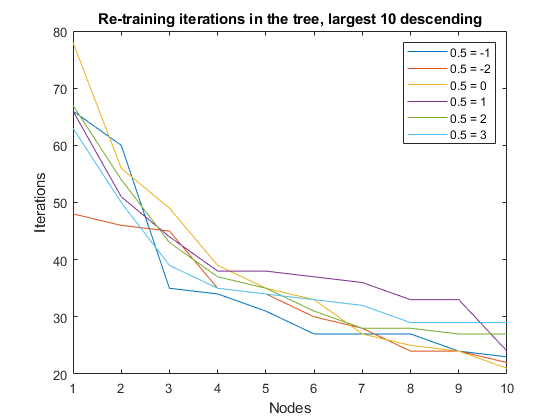
\includegraphics[width=\textwidth]{figures/treeretrainiter10.png}
        \caption{Largest 10 iterations}
        \label{sfig:tree:treeiter10}
    \end{subfigure}
    \hfill
    \begin{subfigure}[b]{.45\textwidth}
        \centering
        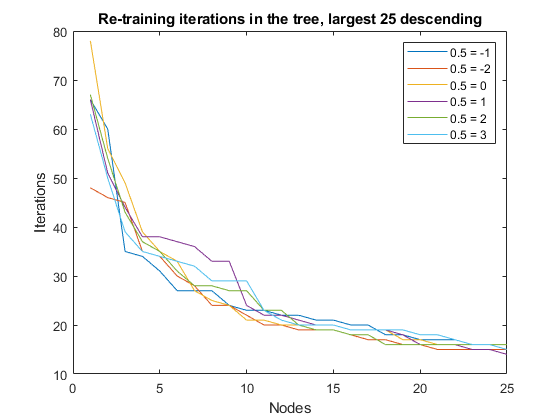
\includegraphics[width=\textwidth]{figures/treeretrainiter25.png}
        \caption{Largest 25 iterations}
        \label{sfig:tree:treeiter25}
    \end{subfigure}
    \caption{Largest tree node iterations in descending order. Excluding full dataset.}
    \label{fig:tree:treeiter}
\end{figure}


\cref{fig:tree:treeiter} show the number of iterations used in the tree nodes, descending from largest to smallest.

%Both node failure and sample loss
\subsection{Failed node generation per branch layer}
Throughout the tree generation process, various samples are removed from further use in the tree.
First, a small number of samples are removed due to a hard requirement of one thousand samples per sample file.
Second, every time a tree node receives less than 20 thousand samples to work with, it is considered finished and subsequently removed.
How this process has developed for each tree generation is a valuable insight into how the tree has formed, and its structure as a whole.
Each tree node can only lose so many samples, meaning that if the tree does not distribute samples enough, it will be very narrow.

\cref{fig:tree:nodefail} shows how many nodes failed to be created on a per branch level.

\begin{figure}  % order of priority: h here, t top, b bottom, p page
  \centering
  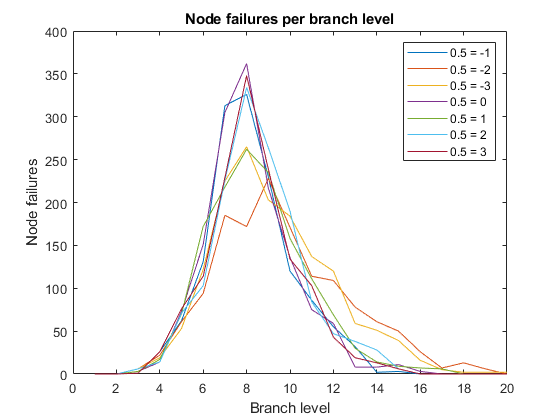
\includegraphics[width=.7\textwidth]{figures/treenodefail.png}
  \caption{Nodes that failed to be created due to insufficient samples in the cache}
  \label{fig:tree:nodefail}
\end{figure}

\cref{fig:tree:sampleloss} shows how many samples were lost during the tree generation process on a per branch level.

\begin{figure}  % order of priority: h here, t top, b bottom, p page
  \centering
  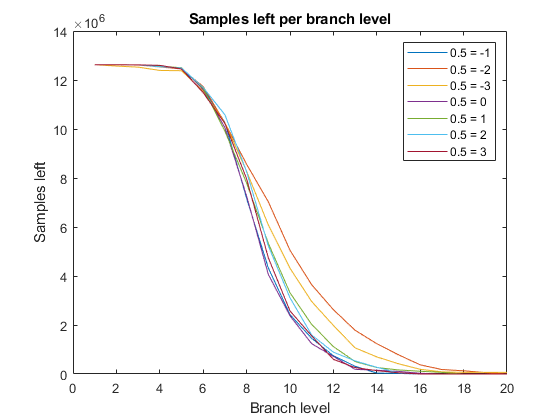
\includegraphics[width=.7\textwidth]{figures/treesampleloss.png}
  \caption{Samples left per branch level over the course of the tree generation}
  \label{fig:tree:sampleloss}
\end{figure}

%Find samples and their groups, compare deep cluster with shallow cluster, see how similar these samples are
\subsection{Comparison between samples classified by the tree}
\label{res:similar}

To compare the performance of the tree generation on the real data, three samples are presented in figures \cref{fig:tree:sample1}, \cref{fig:tree:sample2}, and \cref{fig:tree:sample3}.

The first sample is the most distinct of the three, and splits off from the other two in the tree at the root node, being classified as class 0 while the other two samples are classed as class 2.
The two similar samples follow each other until the end of the tree, with the resulting class combination "210012".

\begin{figure}  % order of priority: h here, t top, b bottom, p page
  \centering
  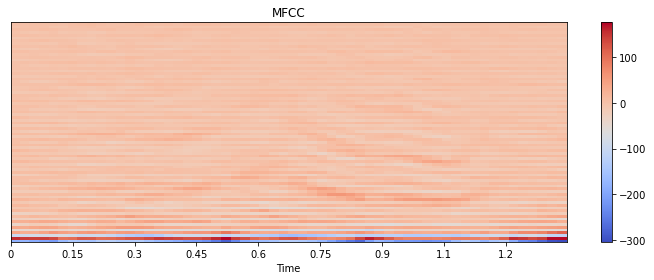
\includegraphics[width=.7\textwidth]{figures/sample1.png}
  \caption{Audio sample 1, English translation: "Kabu, I'm home!"}
  \label{fig:tree:sample1}
\end{figure}

\begin{figure}  % order of priority: h here, t top, b bottom, p page
  \centering
  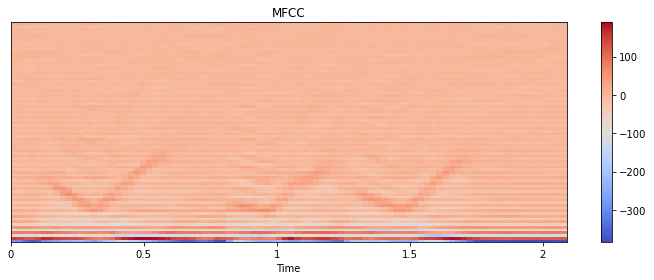
\includegraphics[width=.7\textwidth]{figures/sample2.png}
  \caption{Audio sample 2, English translation: "Nu-uh! I'll go by myself..."}
  \label{fig:tree:sample2}
\end{figure}

\begin{figure}  % order of priority: h here, t top, b bottom, p page
  \centering
  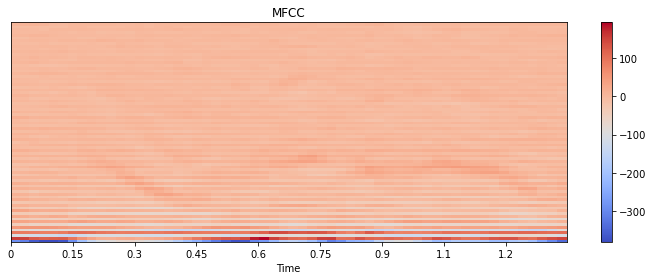
\includegraphics[width=.7\textwidth]{figures/sample3.png}
  \caption{Audio sample 3, English translation: "All right, I'm finished"}
  \label{fig:tree:sample3}
\end{figure}

%Control-specific -3 insight, 0.5-0.2 threshold comparison
\subsection{Control insight}
\cref{ex:tree} used a control function option called "-3" that avoided the re-training process entirely to control for potential faults in the iterative re-training process
The iterative re-training of the other options meant that while training the other options could take hours due to slowly processing the entire dataset; this control option could proceed immediately to the caching stage after the first iteration was trained.
The faster processing time enabled the use of lower cache threshold options, which carry different values than the rest of the trees.
Due to the nature of the softmax layer, with a caching threshold of 0.5, only one node could receive a sample to process.
Using a lower cache threshold enabled the possibility of multiple nodes receiving the same sample, inflating the original dataset throughout the tree generation.

The results of the control group can be compared with the other trees through the combination using the 0.5 cache threshold.
\cref{fig:tree:treecontrolcluster} displays the cache size of the nodes in the control trees.

\begin{figure}
    \centering
    \begin{subfigure}[b]{.45\textwidth}
        \centering
        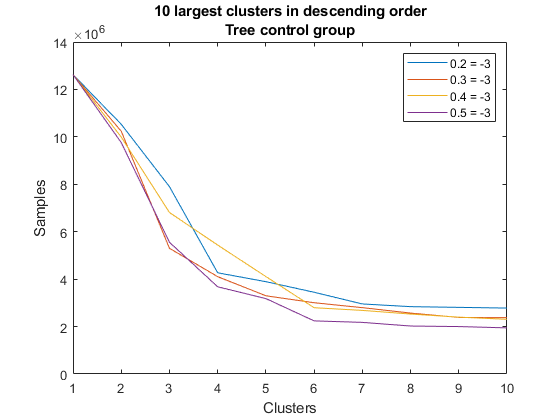
\includegraphics[width=\textwidth]{figures/treecontrolcluster10.png}
        \caption{Largest 10 clusters}
        \label{sfig:tree:treecontrolcluster10}
    \end{subfigure}
    \hfill
    \begin{subfigure}[b]{.45\textwidth}
        \centering
        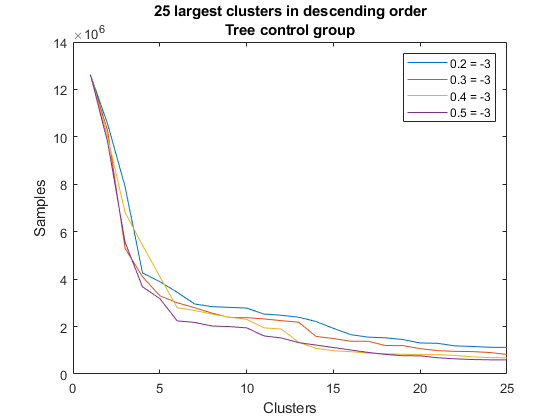
\includegraphics[width=\textwidth]{figures/treecontrolcluster25.png}
        \caption{Largest 25 clusters}
        \label{sfig:tree:treecontrolcluster25}
    \end{subfigure}
    \caption{Largest tree node clusters in the control group, in descending order. Including full dataset.}
    \label{fig:tree:treecontrolcluster}
\end{figure}

\cref{fig:tree:treecontrolnodesample} shows how many nodes failed to be created, and the loss of samples on a per branch level.

\begin{figure}
    \centering
    \begin{subfigure}[b]{.45\textwidth}
        \centering
        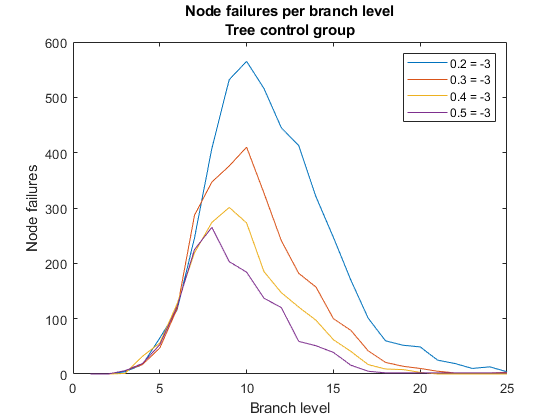
\includegraphics[width=\textwidth]{figures/treecontrolnodefail.png}
        \caption{Node failures}
        \label{sfig:tree:treecontrolnode}
    \end{subfigure}
    \hfill
    \begin{subfigure}[b]{.45\textwidth}
        \centering
        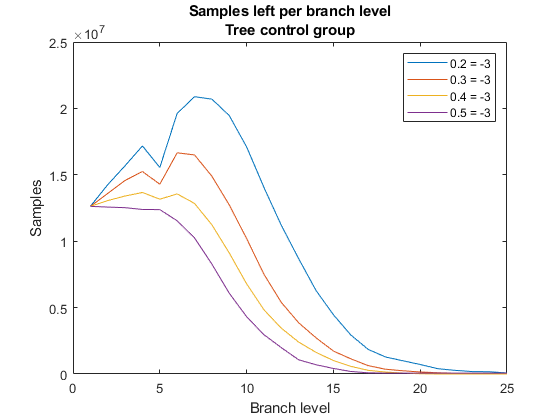
\includegraphics[width=\textwidth]{figures/treecontrolsampleloss.png}
        \caption{Samples left}
        \label{sfig:tree:treecontrolsample}
    \end{subfigure}
    \caption{Node failures and samples left per branch level in the control group.}
    \label{fig:tree:treecontrolnodesample}
\end{figure}

%Trees have a lot more data, processing like with iterative is unfeasible in the time limit left, not sure how good it would be anyway given different purpose
%Cache size per node, descending (tracking the highest nodes in the trees), several graphs with different cutoffs, side by side with one cutoff shorter and one longer (left 10-15, right 35-50?)
%Cache failure count, per branch layer, where cache failed to create a branch
%Cache loss count, per branch layer, how many samples were lost due to failed 0.5 threshold and overflow
%Iteration count to generate node, descending
%Iteration graphs similar to last point in iteration, except for this

%In both iteration graphs, record both hitlist and converted array
